\chapter{Approach Analysis}

\section{Technologies}
	In this section we will give a brief description of the technologies associated to the different approaches we have considered.

	\subsection{Script\#} % (fold)
	\label{sub:subsection_name}
		ScriptSharp \cite{scriptsharp} is a cross-compiler from C\# to JavaScript that is maintained by Nikhil Kothari \cite{nikhilk} from Microsoft. The way ScriptSharp works is that it compiles an entire C\# project to client side JavaScript code.

		The main assembly ScriptSharp.dll is shown in figure \ref{simplifiedOverview} as a simplified dependency diagram with the most relevant assemblies related to our project. When ScriptSharp is used in a regular manner (i.e. not in MiCS) a C\# AST is build from the C\# source code using classes from the Parser and CodeModel namespaces. The ScriptModel namespace contains classes for building the JavaScript AST before the actual script is generated using classes in the Generator namespace.

				\begin{figure}[H]
			\begin{center}
				\centerline{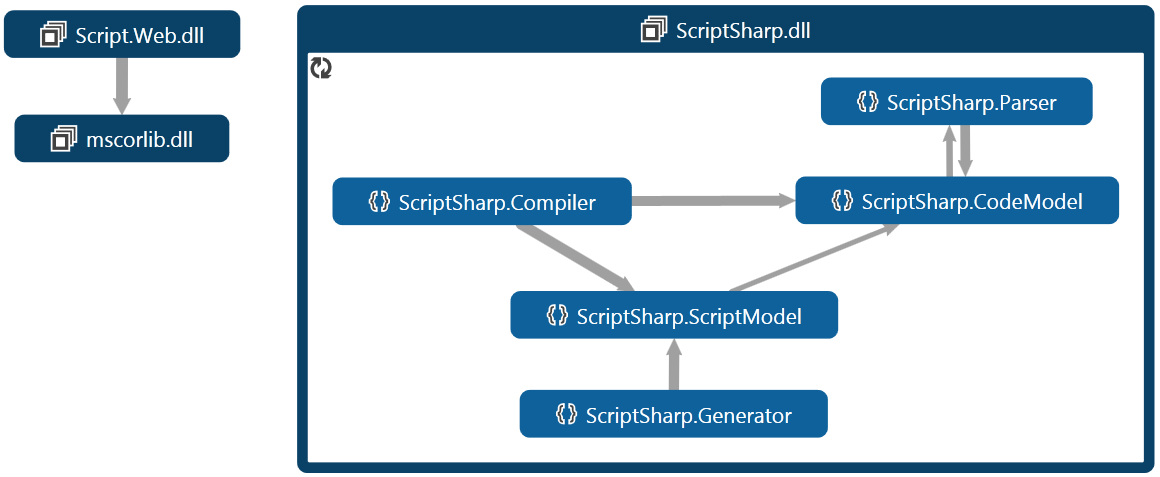
\includegraphics[width=16cm]{resources/images/SimplifiedOverview.png}}
			\end{center}
			\caption{Simplified Script\# architecture overview.}
			\label{simplifiedOverview}
		\end{figure}

		Another important assembly is the Script.Web.dll. This assembly contains classes E.g. for Document Object Model (DOM) representation.

		Script\# defines a modified version of the .NET mscorlib.dll so that the (modified) .NET core type interfaces resembles the equivalent JavaScript objects. E.g. the ScriptSharp defined System.String type has a CharAt(int index) function that doesn’t exist on the original .NET System.String type but that does exist on a JavaScript string object. One benefit of the modified mscorlib.dll is that it makes the C\# compiler able to validate the C\# code that represents JavaScript code entirely (todo: REF to explanation). 

		The modified mscorlib.dll file is referenced in one’s Visual Studio project (instead of the original one) when a new ScriptSharp project is created. When a ScriptSharp project is compiled a JavaScript file will be generated. This JavaScript file can then be used in other projects (E.g. a Web Forms web application).
	% subsection subsection_name (end)

	\subsection{Microsoft Roslyn} % (fold)
	\label{ssub:microsoft_roslyn}
		todo
	% subsection microsoft_roslyn (end)

	\subsection{Code Quotations} % (fold)
	\label{ssub:code_quotations}
		todo
	% subsection code_quotations (end)

	\subsection{Expression Trees} % (fold)
	\label{ssub:expression_trees}
		todo
	% subsection expression_trees (end)

	\subsection{Internal DSL} % (fold)
	\label{ssub:internal_dsl}
		todo
	% subsection internal_dsl (end)

\section{Stages when going from .NET Language to JavaScript} % (fold)
\label{sec:stages_when_going_from_net_language_to_javascript}
	Before discussing different approaches it make sense to clarify the possible stages in the process of “going” from host to target language. The process (displayed in figure \ref{stages}) moves from left to right and possibly skips stages on the way.

				\begin{figure}[H]
			\begin{center}
				\centerline{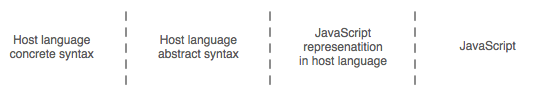
\includegraphics[width=12cm]{resources/images/stages.png}}
			\end{center}
			\caption{Possible approach stages}
			\label{stages}
		\end{figure}

	The host language concrete syntax, whether an internal DSL or the host languages native syntax, is what the end user will be utilizing. From this concrete syntax a host language abstract syntax tree (hereinafter AST) can be generated. This AST can be traversed in order to map the host language AST to a JavaScript representation (typically also an AST) in the host language. Finally, JavaScript can be generated from the JavaScript AST.
% section stages_when_going_from_net_language_to_javascript (end)

\section{Possible Approaches} % (fold)
\label{sec:possible_approaches}
	todo text

					\begin{figure}[H]
			\begin{center}
				\centerline{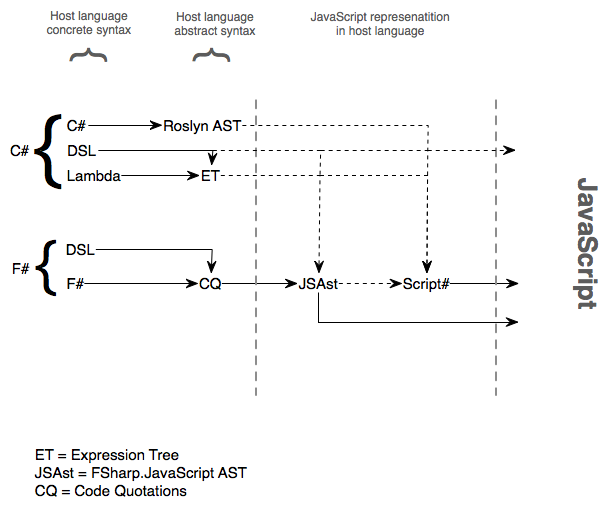
\includegraphics[width=14cm]{resources/images/DSLv2.png}}
			\end{center}
			\caption{Map of possible approaches.}
			\label{approachMap}
		\end{figure}

	\subsection{Internal DSL Approaches} % (fold)
	\label{ssub:internal_dsl_approaches}

		The Internal DSL approaches has been separated into two categories. The first where the DSL is used to build a host language AST which later can be mapped to a target language AST. The second where the target language AST is created directly (i.e. the Host Language Abstract Syntax stage is skipped). One significant difference in these two approaches has to do with the possibility of executing code both on server side and client side. When generating the host language AST before mapping to the target language AST its easier to also execute the code in the host language context through dynamic compilation of the host language AST (this approach is discussed in xx TODO).
	
		\subsubsection{Internal DSL Directly to JavaScript AST} % (fold)
		\label{sub:internal_dsl_directly_to_javascript_ast}
		
			When utilizing an internal DSL one would need classes for representing primitive types, expression, statements etc. All the target language features that one will make available needs to be mapped to a DSL representation. Every DSL call would then instantiate an equivalent target language AST node.

			One thing important to consider when creating a DSL representing a different language is its syntax. The DSL syntax should resemble the target language concrete syntax so that the DSL is easily utilized by the target users. At the same time, it should make the verbose instantiation (see example below) of host abstract syntax less cumbersome.

			todo: redo code example

		% subsection internal_dsl_directly_to_javascript_ast (end)

		\subsubsection{C\# DSL} % (fold)
		\label{sub:cs_dsl}

			To approach the project initially we did some experiments with a DSL (in C\#) that created a JavaScript AST directly (i.e. the Host Language Abstract Syntax stage was skipped) (See appendix for class diagram and maybe description of scope / block handling mechanism etc.). Using helper factory methods (to create AST nodes), operator overloading and a scope and block handling mechanism (utilizing Statement Lambdas) one can arrive at a DSL syntax that could be somewhat compared to concrete syntax (see example below).

			todo: redo code example

			There are though different problems with this approach. First of all the syntax is a bit different from any of the existing syntaxes, i.e. it doesn’t exactly resemble regular C\# or JavaScript. This implies that there will be a learning effort before the DSL can be used. Furthermore the syntax is a bit verbose and not optimal when it comes to readability.
		
		% subsection subsection_name (end)

		\subsubsection{F\# DSL} % (fold)
		\label{sub:fs_dsl}
			One problem with the C\# DSL implementation is that the initial declaration and assignment of the variable “i” is done using “=” operator where any subsequent assignments should be done using the ``Assign(...)'' method (or possibly through overloading an existing operator e.g. ``\%=''). The main reason for this is that it is not possible to override the assignment operator in C\# (QUOTATION). This is a critical problem because if the regular C\# assignment operator ``\='' was used incorrectly by mistake it would not trigger any exceptions and therefore cause a difficult to debug error.  The example below shows exactly this. The variable “i” is assigned in an incorrect manner after its initial declaration according to the DSL syntax.

			todo: redo code example

			This would not be an issue in F\# as the assignment operator could be overloaded. Furthermore it is even possible to implement new operators consisting of one or more characters from a given set of characters, consequently making it possible to implement some special JavaScript operators such as strict equal (===).

			One problem though with the F\# DSL approach is the fact that the F\# native syntax and programming paradigm (e.g. the use of immutable types) is radically different from that of JavaScript (and C\# for that matter). This would imply an even bigger learning curve according to our target user as one would have learn the F\# syntax and programming paradigm together with the DSL. Even if F\# was the language of choice there are other powerful language features (Code Quotations) that might bias you toward a different approach (see section ``Using F\# Code Quotations'').
		% subsection fs_dsl (end)

		\subsubsection{DSL to Host AST} % (fold)
		\label{sub:dsl_to_host_ast}
			To accommodate the mixed side execution goal one possibility in C\# is to utilize Expression Trees. With this approach the DSL would build a host language AST represented as an Expression Tree which hereafter could be mapped to JavaScript. The host language AST can also be compiled into host language executable code using the Compile() feature (todo: QUOTATION) on Expression Trees. With an F\# DSL approach a similar pattern could be achieved with Code Quotations (the Expr type). A more straightforward solution to the mixed side execution goal would though be to not use a DSL. Instead one would use the concrete syntax of host language. Then utilize dynamic compilation to retrieve the host language AST which is what we’ll discuss in the next section (todo: REF ``Using Roslyn'').
		% subsection dsl_to_host_ast (end)
	% subsubsection internal_dsl_approaches (end)


	\subsection{Host Language Approaches} % (fold)
	\label{sub:host_language_approaches}
		Instead of using an internal DSL, tools (or in some cases language features) exist to generate AST’s from native host language code. These can be traversed and processed as desired by the programmer.

		As tools handle the generation of a host language AST, the workload imposed on the programmer by using this approach is considerably smaller than using e.g. an internal DSL. When using an internal DSL it is up to the programmer to implement a library that represents its concrete syntax.

		The workload is also lightened on the end user. When using tools to generate a host language AST it is possible for the end user to write native code and have it converted to JavaScript instead of having to learn how to use a new library.

		As the host language AST is generated from native host language code it is possible to use the same code on both client side and server side, as the client side code is generated from the server side code. This is very useful with cases such as form validation as it is not necessary for the end user to write the same logic in two different languages. Furthermore, it allows the end user to generate client side code reusing code from previous C\# projects.

		Another benefit of using native host language code, is the possibility of testing on server side. As the code is able to run and evaluate on server side, the end user won’t have to write tests in two different languages as the unit testing framework has effectively also been applied to the client side code.

		One disadvantage of using an AST generated from a native host language is that there are no restrictions on what the end user might do. The scope of the project is set by our case study, and as such, our solution will be unable to convert every single construct of an entire language. Should the end user choose to use a language construct that our solution does not support, it will result in a (server-side) runtime error, whereas a DSL would already discover this on compile time. The reason for this is the intrinsic limiting nature of a DSL (todo: REF BOOK: Domain Specific Languages).

		\subsection{Using F\# Code Quotations} % (fold)
		\label{sub:using_fs_code_quotations}
		
			Code Quotations is a built-in feature in the F\# language which lets a developer generate an abstract syntax tree that represents the corresponding F\# code. Code Quotations cover the entire F\# language, meaning that theoretically all F\# constructs can be mapped to a corresponding JavaScript construct.

			The main disadvantage of using Code Quotations is that they require the end user to know a different language from the one in which ASP.NET WebForms Applications are typically written (C\#). This would probably not be a very great barrier if the syntax of the language didn’t vary as much as F\# does from C\#. Also, C\# and JavaScript are somewhat similar in syntax, whereas F\#'s and JavaScripts syntaxes are beyond comparison.
		% subsection using_f#_code_quotations (end)

		\subsection{Using C\# Expression Trees} % (fold)
		\label{sub:using_cs_expression_trees}
			Expression Trees is a built-in feature in the C\# (and Visual Basic) language that “represents code in a tree-like data structure, where each node is an expression, for example, a method call or a binary operation” (REF MSDN). Expression Trees are often used with LINQ to build dynamic queries, which can be useful when fetching data from a database with filters specified by the user (these filters may be provided through a user interface). Expression Trees can be generated from lambda expressions, and thus it is possible to retrieve a representation of simple pieces of code, such as the following:

			todo: code example: Func<int, int, bool> function = (a, b) => a > b

			or more sophisticated ones such as LINQ queries.  A major pitfall using Expression Trees is that they cannot be generated from lambda statements, which prevents the possibility of generating AST’s from blocks of code.
		% subsection using_C\#_expression_trees (end)

		\subsection{Using Roslyn} % (fold)
		\label{sub:using_roslyn}
			Roslyn is a Microsoft project that exposes the C\# and Visual Basic compilers as services. Even though the two are alike, we will focus on C\#. As with F\# Code Quotations, Roslyn is able to generate an AST from C\# source code, and as with Code Quotations, Roslyn is full fidelity (REF) which means that all C\# constructs can be recognized and parsed into syntax nodes. In fact, the AST generated by Roslyn contains every single character of the original source code, down to the last piece of whitespace. Thus, Roslyn combines the advantages of Code Quotations and Expression Trees by allowing the generation of an AST from every C\# construct (including blocks), and avoiding the unfamiliar F\# syntax.
		% subsection using_roslyn (end)
	% subsection host_language_approaches (end)

% section possible_approaches (end)

\section{Deciding on Approach} % (fold)
\label{sec:deciding_on_approach}
	todo: text

						\begin{figure}[H]
			\begin{center}
				\centerline{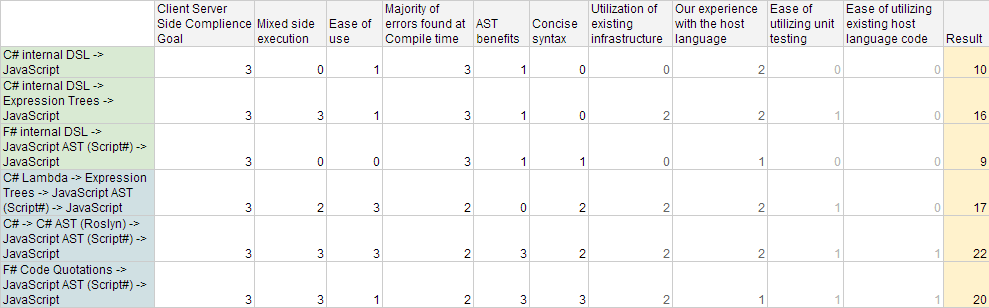
\includegraphics[width=14cm]{resources/images/ApproachMatrix.png}}
			\end{center}
			\caption{Approach Matrix.}
			\label{approachMatrix}
		\end{figure}

	todo: more text
% section deciding_on_approach (end)